\chapter{Ab-initio Studies of Exciton Interactions of Cy5 Dyes }
\label{chap:ab-initio}

The following chapter was published in Journal of Physical Chemistry A in 2018 under authors Jenny W. Fothergill, Andres Correa Hernandez, William B. Knowlton, Bernard Yurke, and Lan Li. My contributions to this paper were all DFT, python, and java calculations with guidance from Drs Li and Yurke, data curation and analysis with input from all authors, all figure creation, and all draft writing with the help of feedback from all authors.

\section{Abstract}

The excited state properties of cyanine dyes and the orientations of their aggregates were studied using density functional theory (DFT). The effects of exchange-correlation functional and solvent model on the absorption spectrum of Cy5 was investigated. Using the 6-31+G(d,p) basis set and B3LYP exchange-correlation functional with IEF-PCM (water) solvent, the predicted spectrum achieved a maximum absorbance within 0.007 eV of experiment. An in-house program based on the theoretical model of Kühn, Renger, and May (KRM), which predicts the orientation of dyes within an aggregate from its absorbance and circular dichroism (CD) spectra or vice versa, was used to investigate the orientation of an experimentally observed dimer. The absorbance spectrum predicted using the KRM model of the dimer structure optimized with the 6-31+G(d,p) basis set, $\omega$B97XD exchange-correlation functional, and IEF-PCM (water) solvent agrees with experimental data. 

\section{Introduction}
Chromophore aggregates in the light-harvesting complexes of photosynthetic organisms have been shown to exhibit exciton delocalization, in which an electron-hole pair is delocalized over spatially separated chromophores \cite{Engel2007, Collini2010a, Fassioli2014}. Exciton delocalization plays a role in the energy transfer to the reaction center in photosynthesis and was first observed in nonbiological molecular crystals \cite{Frenkel1931, Frenkel1931a, Davydov1964, Eisfeld2007, Eisfeld2006a}. Early steady-state absorption measurements suggested exciton delocalization was present in chlorophyll from spinach photosystem I \cite{Philipson1972}. Later, femtosecond two-dimensional spectroscopy was used to observe the indicative quantum “beating” between chromophores in bacteriochlorophyll at 77K, a result that was later confirmed at room temperature \cite{Marcus1965a, Lloyd2011a}.  These excitonic phenomena are of considerable interest due to their potential for applications in the realms of solar energy harvesting and quantum optics \cite{Smyth2012a, Rossi2004, Childs2013a}. A signature of exciton delocalization in dye aggregates is the shifted absorption maxima (relative to the monomer) due to molecular transition dipole interactions. When two chromophores come close enough that their transition dipoles interact, the excited state energy is split. Two commonly formed types of aggregate are known as J- and H- aggregates \cite{Wurthner2011}. J-aggregates, named after the chemist E. E. Jelley, display a narrow, intense, bathochromic absorbance (i.e., red shift) with nearly resonant fluorescence, while H-aggregates display a hypsochromic shift (i.e., blue shift) in absorbance maxima and quenched fluorescence as explained by the molecular exciton theory of Kasha \cite{Kasha1963}. 
\begin{figure}[h!]
    \centering
    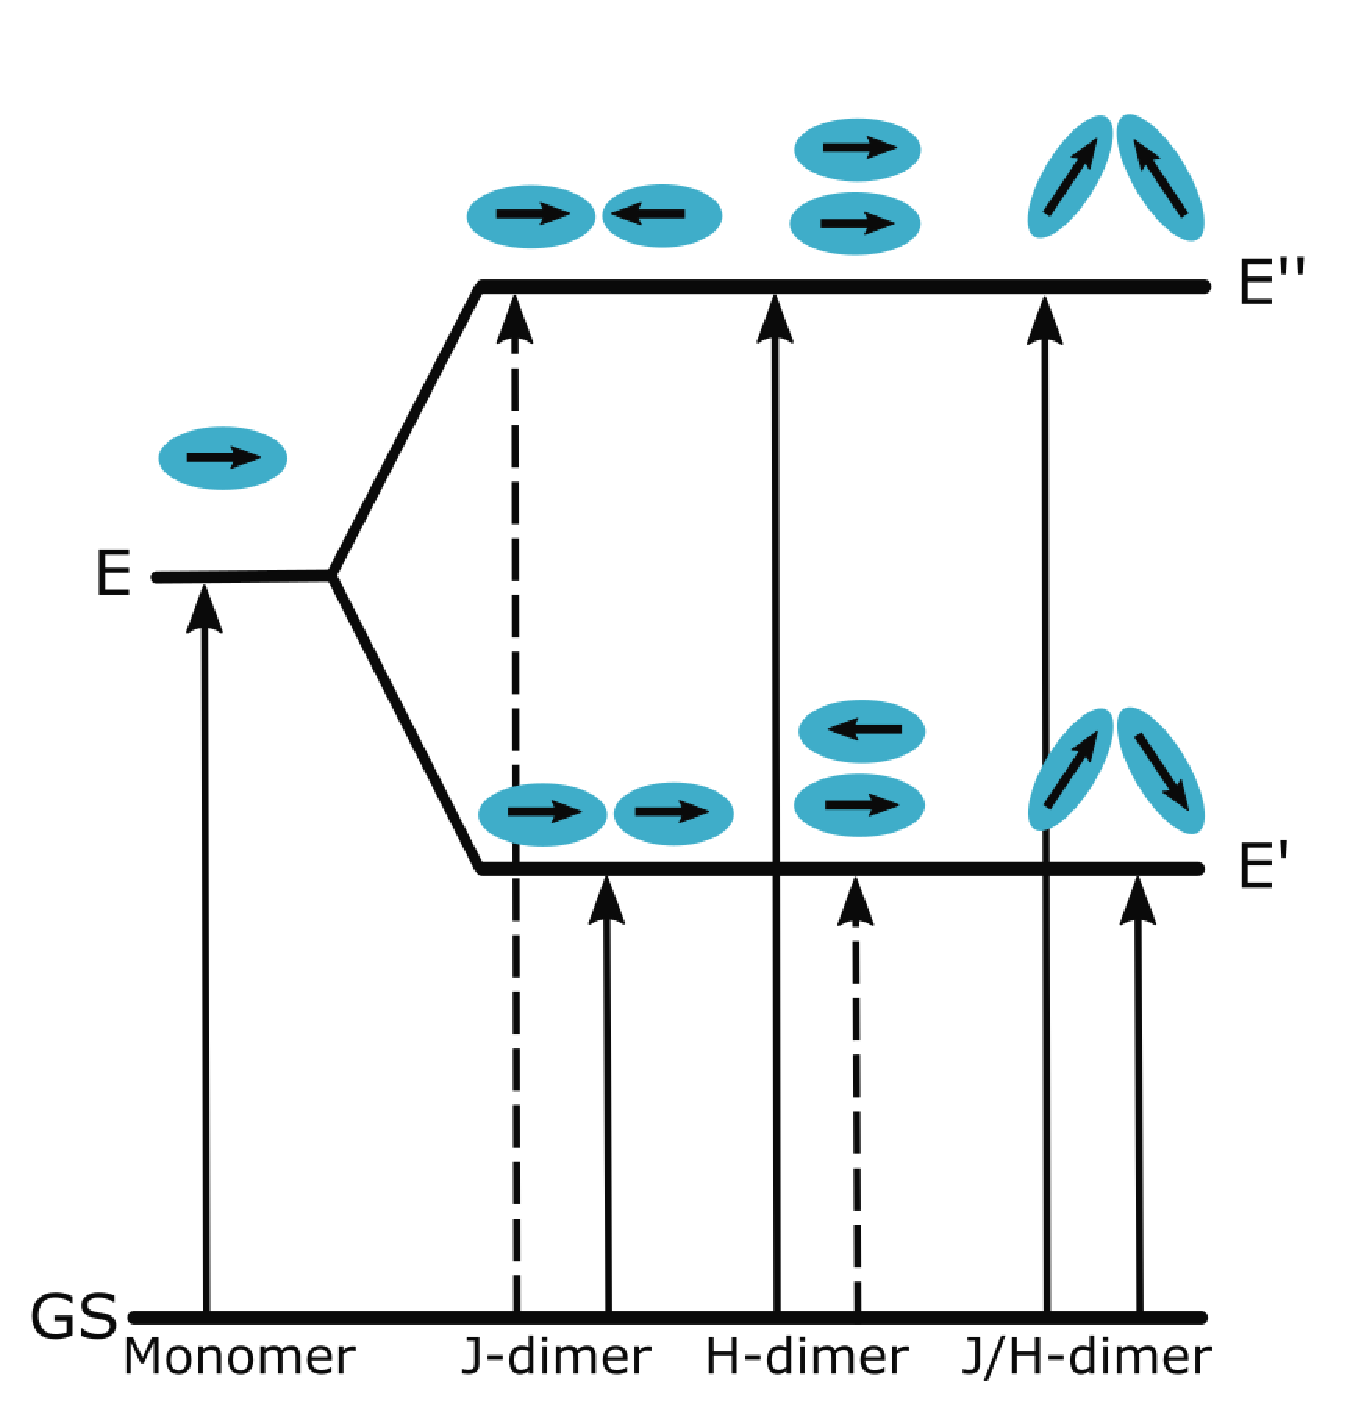
\includegraphics[width=0.8\linewidth]{figures/pub1/energy-diagram.pdf}
    \caption{Energy diagram based on molecular exciton theory of Kasha showing the excitation pathways for the J-dimer, H-dimer, and oblique dimer relative to the monomer \cite{Wurthner2011}. The allowed (solid) and forbidden (dashed) transitions result from the orientations of the molecular transition dipole moments.}\label{energydiagram}
\end{figure}
\autoref{energydiagram} illustrates the energy splitting and allowed states of different dye dimers. The transition dipole moment is assumed to be parallel to the long axis of the dye molecule. The selection rules for light absorption involve taking the vector sum of the transition dipoles, so only transitions with net non-zero vectors are allowed. Oblique aggregates, in which the alignment of the transition dipole moments of the dyes is at some angle between the H- or J- configurations, have allowed transitions to both the higher and lower energy states, so the absorbance spectra show Davydov splitting of their absorbance maxima \cite{Davydov1964}. Due to their excitonic properties, dye aggregates have been proposed to be used for light harvesting and excitonic quantum computing applications \cite{Scholes2012a, Scholes2011b, Scholes2011a, Romero2017a}. However, the chromophores must be precisely spaced in order to achieve predictable exciton delocalization behavior as small changes in the orientation of the chromophores will cause large shifts in the absorption spectra.

Recently, cyanine dyes covalently incorporated into duplex DNA have been studied for their exciton delocalization properties that include J- and H-aggregate behavior and Davydov splitting that manifest as red shifts, blue shifts, and simultaneous red and blue shifts in absorbance, respectively, as compared to the dye monomer. The self-assembly properties of DNA can bring dyes within separation distances that induce shifts in the absorption maxima. Using DNA as a scaffold allows for manipulation of the orientation of cyanine dye molecules. DNA nanotechnology enables the precise construction of nanodevices due to the self-assembly of nucleic acids determined by Watson-Crick base pairing. The use of DNA as a building material has demonstrated precise control of 2D and 3D nanoscale shapes \cite{rothemund06, Ke2012a}. It has been shown that Cy5 dimers covalently bound into the sugar-phosphate backbone of duplex DNA adopt a J-dimer configuration in 100 mM sodium chloride \cite{Markova2013}. Another study found that Cy3 dimers covalently attached to DNA showed H-dimer absorbance in which the intensity varied with base-pair separation distance and the rigidity of the DNA scaffold \cite{Nicoli2016b}. The exciton-coupling strength of Cy3 dimers in double-stranded DNA has been found to decrease with an increase in temperature \cite{Kringle2018b}. It has also been found that varying the salinity of a solution containing Cy5 in DNA with magnesium chloride (from 0 mM to 100 mM) as well as the DNA concentration resulted in a conformational change from a J- dimer to H- tetramer configuration \cite{Cannon2017}. The relative orientation of the dyes in the DNA scaffold has been investigated by fitting the absorption and circular dichroism (CD) spectra using an in-house program based on the theoretical model of Kühn, Renger, and May (KRM) \cite{Cannon2017, Cannon2018, Kuhn1996}. In this model, the dominant vibrational mode of the electronic ground state and the electronic excited state of each molecule in the aggregate is treated non-perturbatively by including its Hamiltonian in the system Hamiltonian that is diagonalized on a truncated Hilbert space in order to obtain the system energy eigenvalues. To go beyond the approximation in which the exchange interaction arises from point dipoles, the program, from here on referred to as the KRM code, treats the interaction using the extended dipole model \cite{Czikklely1970}. In this manner, the program is able to more accurately model aggregates of rod shaped molecules, like Cy5, for which nearest neighbor distances can be shorter than the length of the molecules. Cannon et al. used the KRM code to find the orientation of the chromophores by varying the input orientations and fitting parameters until a good fit was obtained between the theoretical and experimental spectra \cite{Cannon2017, Cannon2018}. Having determined the values of the fitting parameters for Cy5, the KRM code can be used to predict the absorbance and CD spectrum of a given Cy5 aggregate structure. Further detail about the methods implemented in the code can be found in \citet{Cannon2017}. 

\begin{figure}[h!]
    \centering
    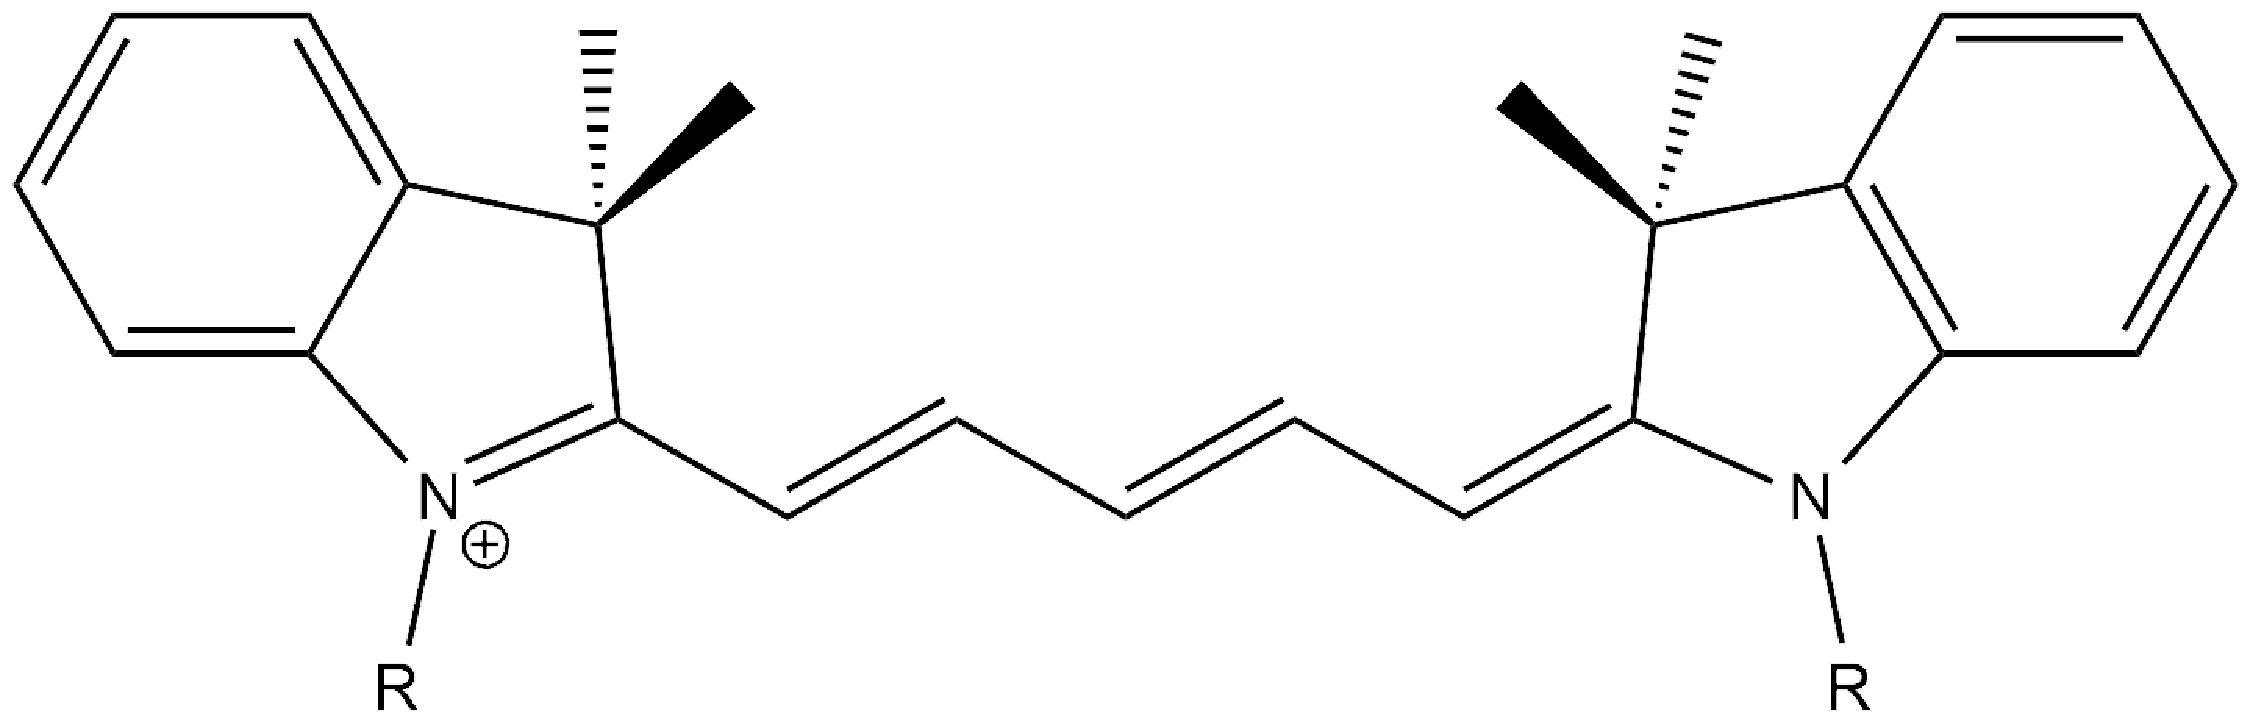
\includegraphics[width=0.8\linewidth]{figures/pub1/Cy5.pdf}
    \caption{The molecular structure of Cy5 (or 1-1'-dimethyl-3,3,3',3'-tetramethylindocarbo-cyanine). Linkers are attached at R groups: for H-dimers and monomer, R = methyl, for oblique dimer, R = propyl chain.}\label{cy5}
\end{figure}
This paper investigates the excited state and intermolecular Cy5 (see \autoref{cy5} for structure) dye interactions using ab-initio density functional theory (DFT)-based approach. Determining the position and orientation of these molecules is a vital first step to study their excitonic behavior. This work is in support of a previously published article in which the orientation of dyes covalently bound to duplex DNA was investigated by analysis of the absorption and circular dichroism spectra using the KRM model \cite{Cannon2017}. The dimer orientation predicted by Cannon et al. for a Cy5 dimer in duplex DNA in 0 mM MgCl2 from analysis with the KRM code of the absorbance and circular dichroism data (this dimer structure is from here on referred to as the oblique dimer) was also optimized using different exchange-correlation functionals \cite{Cannon2017}. The predicted spectra of the optimized oblique dimer structures using the KRM code were compared to the experimental spectrum obtained by \citet{Cannon2017}. Vibrationally resolved absorbance spectra for the Cy5 monomer were generated using each exchange-correlation functional and compared to the experimental spectra. The computational results advanced our understanding of exchange-correlation functional effect on the structural stability and excitonic phenomenon of the Cy5 materials. 

For the Cy5-DNA materials system to be considered as a viable candidate for excitonic applications, control of position of Cy5 dyes in different DNA assemblies must be demonstrated. In our work, DFT-based electronic structure calculations helped determine the orientation of Cy5 dyes in DNA at the ground state. TD-DFT modelled a system in the excited state, revealing the effect of exchange-correlation functional and solvent on the absorbance spectra.

\section{Methods}

All ab-initio calculations were performed via the Gaussian09 quantum chemistry package \cite{Frisch2009a}. Molecules were first optimized using the semi-empirical PM6 method \cite{Stewart2007}. These structures were then optimized to a residual force of 4.50x10-4 Hartree/Bohr (2.31x10-2 eV/\AA) using the Kohn-Sham formulation of DFT with the B3LYP, CAM-B3LYP, or $\omega$B97-XD hybrid exchange functionals and 6-31+G(d,p) basis set \cite{Becke1993c, Yanai2004, Chai2008a, Petersson1988a, Petersson1991a}. B3LYP is a three-parameter hybrid, combining Hartree-Fock, GGA, and LDA with no long-range or dispersion correction \cite{Becke1993c}. CAM-B3LYP also considers long-range correction by the Coulomb attenuating method \cite{Yanai2004}. $\omega$B97-XD has both long-range and damped empirical dispersion corrections \cite{Chai2008a}. The effect of basis set extension was also investigated using the 6-311++G(2df,2pd) basis set. These basis sets and exchange-correlation functionals were chosen based on a study which found them to work well for the Cy5-DNA system \cite{Maj2013}. Because the research focus is on the excited state energies, the diffuse functions (represented by +) and the polarization functions (represented by the p, d, or f orbital designation) in the basis set were used to better approximate the higher energy molecular orbitals. All solvated structures were optimized using the polarizable continuum model of water solvent using the integral equation formalism (IEF-PCM) \cite{Tomasi2005c}. Structures were confirmed to be minima on the potential energy surface by the lack of negative vibrational frequencies.

The terms flipped and stacked denote the position of the tertiary amine groups in the dimers: stacked refers to the amine groups of each dye molecule being on the same side while flipped refers to the amine groups being on opposite sides (see \autoref{h-flipstack}). The initial positions of the flipped and stacked H-dimer were chosen by placing the centers of the molecules within 1 nm of each other but no closer than 5 \AA because any closer is not physically likely to occur. The atoms in the H-dimer were fully geometrically relaxed. 
\begin{figure}[h!]
    \centering
    \includegraphics[width=0.8\linewidth]{figures/pub1/h-flipstack-ab.pdf}
    \caption{The initial structures for the flipped (a) and stacked (b) Cy5 H-dimers. The blue atom represents the nitrogen in the amine group while carbon is in grey and hydrogen is in white.}\label{h-flipstack}
\end{figure}

The initial position of the oblique dimer was obtained by matching the dimer position with the orientation vectors obtained by Cannon et al. using the KRM code \cite{Cannon2017}. In the experiments of Cannon et al., the oblique dimer was covalently bound into DNA, so to model this situation, the initial orientation of the oblique dimer from the KRM code was covalently bound into the DNA backbone with propyl linkers and optimized using the universal force field (UFF) in the Avogadro molecule editor \cite{Rappe1992e, Hanwell2012}. Then, the position of the terminal carbon atom on the linker group was frozen to simulate binding to DNA, and the DNA was removed to reduce computational time before optimization using PM6 followed by DFT optimization with a hybrid functional. 

To investigate the effect of solvent on the excited state energies, a linear response formalism which adds the solvent terms to the excited state equations was employed, and the geometry of the lowest excited state was optimized with IEF-PCM water solvent. To account for the Duschinsky effect (i.e., the change in vibrational modes upon electronic transition), the Adiabatic Hessian approach was used to expand the excited state potential energy surface around the equilibrium excited state geometry \cite{AvilaFerrer2012b, Adamo2013b}. To obtain a vibrationally resolved absorption spectra the magnitude of the transition dipole moment between vibrational levels in the ground and excited states was approximated using the Franck-Condon (FC) with and without the Herzberg-Teller (HT) approximation for comparison \cite{Baiardi2013a, Sharp1964a, Franck1926a, Condon1926, Herzberg1933}. The resulting stick spectra were broadened using Gaussian functions with a half-width at half-maximum (HWHM) of 300 cm-1.

\section{Results and Discussion}

\autoref{tab:cy5-solvation} and \autoref{tab:h-solvation} show the solvation energy for the Cy5 monomer and H-dimer and the dye-dye interaction energy of the H-dimers in consideration of various basis set and exchange-correlation functional combinations. The solvation energy is calculated as follows:
\begin{equation}\label{esol}
    E_{sol}=E_{T}-E_{v}
\end{equation}
where $E_{T}$ is the energy of the solvated molecule and $E_{v}$ is the energy of the relaxed molecule structure in vacuum. The interaction energy of the dimer is calculated as follows:
\begin{equation}\label{eint}
    E_{int}=E_{dimer}-2\times E_{monomer}
\end{equation}
where $E_{dimer}$ is the energy of the dimer and $E_{monomer}$ is the energy of the monomer. 

\begin{table}[h]
\centering
\caption{Solvation energy of relaxed Cy5 monomer for given basis sets and exchange-correlation (xc) functionals} \label{tab:cy5-solvation}
\begin{tabular}{llc}
\hline
Basis Set & xc-functional & Solvation Energy (eV) \\ \hline
6-31+G(d,p) & B3LYP & -1.488 \\ 
6-31+G(d,p) & CAM-B3LYP & -1.501 \\ 
6-31+G(d,p) & $\omega$B97-XD & -1.506 \\ 
6-311++G(2df,2pd) & B3LYP & -1.477 \\ 
6-311++G(2df,2pd) & CAM-B3LYP & -1.492 \\ 
6-311++G(2df,2pd) & $\omega$B97-XD & -1.493 \\ 
\end{tabular}
\end{table}

\begin{table}[h]
\centering
\caption{Solvation energy and interaction energy of relaxed Cy5 H-dimers (flipped and stacked) for given basis sets and exchange-correlation (xc) functionals} \label{tab:h-solvation}
\begin{tabular}{lllp{15mm}p{20mm}}
\hline
Structure & Basis Set & xc-functional & Solvation Energy (eV) & Interaction Energy (eV) \\ \hline
\multirow{6}{*}{H-dimer (flipped)} & 6-31+G (d,p) & B3LYP & -4.234 & 0.002 \\ 
 & 6-31+G (d,p) & CAM-B3LYP & -4.343 & -0.039 \\ 
 & 6-31+G (d,p) & $\omega$B97-XD & -4.460 & -0.636 \\ 
 & 6-311++G (2df,2pd) & B3LYP & -4.104 & 0.008 \\ 
 & 6-311++G (2df,2pd) & CAM-B3LYP & -4.334 & -0.025 \\ 
 & 6-311++G (2df,2pd) & $\omega$B97-XD & -4.427 & -0.572 \\ \hline
\multirow{6}{*}{H-dimer (stacked)} & 6-31+G(d,p) & B3LYP & -4.413 & -0.003 \\ 
 & 6-31+G(d,p) & CAM-B3LYP & -4.638 & -0.069 \\ 
 & 6-31+G(d,p) & $\omega$B97-XD & -4.690 & -1.054 \\ 
 & 6-311++G(2df,2pd) & B3LYP & -4.239 & 0.009 \\ 
 & 6-311++G(2df,2pd) & CAM-B3LYP & -4.624 & -0.044 \\ 
 & 6-311++G(2df,2pd) & $\omega$B97-XD & -4.663 & -1.033 \\ \hline
\end{tabular}
\end{table}

The solvation energy is used as a qualitative measure to determine which dye orientation will be more stable as the experiment we aim to support takes place in aqueous solution \cite{Cannon2017}. The more negative the solvation energy, the more energetically favorable for the constituent to exist in the solvent. \autoref{tab:cy5-solvation} and \autoref{tab:h-solvation} show that the solvation energy of the dimer is more negative per chromophore than that of the monomer, suggesting that the dimer structure would be more energetically favorable in a polar solvent such as water. We suggest the reason for this is the reduction of hydrophobic interactions with the solvent. The monomer calculations show no significant difference in either structure or solvation energy as exchange-correlation functional varies. For the dimer structures, however, the way in which the functional models consider long-range and dispersion interaction differs and thus impacts the results. Compared to the flipped structure, the stacked H-dimer structure overall has more negative solvation energy because in the optimized geometry this dimer is more compact and thus required a smaller cavity in the solvent. 

The interaction energy provides insight into the strength of the intermolecular interaction of the two dyes. \autoref{tab:h-solvation} shows that the interaction energy between the H-dimers using B3LYP is very small or even positive suggesting that this functional underestimates the intermolecular dye interactions because similar cationic cyanogen dyes are known to aggregate in aqueous solution \cite{Herz1974, VonBerlepsch2000a, Friedl2016a}. Considering the long-range correction (CAM-B3LYP) in the exchange-correlation functional lowers the energy, but adding dispersion corrections ($\omega$B97-XD) results in the lowest energy (i.e., the most favorable interaction) for both the flipped and stacked H-dimer. The interaction and solvation energies indicate that the stacked H-dimer is more energetically favorable, i.e., more stable, than the flipped structure, even though stacking the methyl groups could result in steric hindrance; potentially, favorable pi-stacking of the aromatic rings contributes to the lower interaction energy. 

As Cy5 is a cationic dye, a preliminary investigation into the effect of the presence of an explicit (chlorine) counter ion was done (see Supporting Information \autoref{tab:cl-energies}). However, analysis with the KRM code suggests that the oblique dimer structure which was relaxed with counter ions is not a better fit to experiment (see \autoref{spectra-cl}).

Comparison of the solvation energy or the interaction energy of the H-dimer structures optimized using the same exchange-correlation function and either the small (6-31+G(d,p)) or large (6-311++G(2df,2pd)) basis sets shows that these energies do not differ between basis sets. A good agreement between the relaxed dimer structures within the same exchange-correlation functional and between basis sets further confirms that the basis set superposition error (BSSE) is negligible in the small basis set. (For a detailed orientation of each dye within the dimer structures, see \autoref{tab:h-stacked-orientation} and \autoref{tab:h-stacked-orientation}.) Finally, this similarity of the optimized structures between basis sets can be visualized using the absorbance spectra predicted by the KRM code, where small changes in dye orientation will induce large shifts in the absorbance (see \autoref{spectra-bsse}). 

To compare the spectra, and thus the difference between the dimer structures, the root mean square error (RMSE) is provided as a measure of the difference between two absorbance data as follows:
\begin{equation}\label{rmse}
    RMSE= \sqrt{\frac{\sum_{i=1}^n (y_{1i}-y_{2i})^2}{n}}
\end{equation}
where $y_{1}$ and $y_{2}$ are the y-axis (absorbance) values corresponding to the first and second data sets and $n$ is the number of points. The lower the RMSE, the more similar the spectra, and if the two data sets are equal, the RMSE will be zero. 

Including the DNA in the DFT calculation makes the system unmanageably large, so investigation of the effect of the DNA scaffold on the Cy5 dimer structure was done in stages. First, the initial structure of the oblique dimer, which was experimentally observed in duplex DNA, was designed to fit the orientation vectors found by Cannon et al. using the KRM code \cite{Cannon2017}. As confirmation, following the UFF relaxation of the dye dimer in DNA structure, the vector fit of the relaxed dimer structure was re-entered into the KRM code to ensure that the predicted spectrum continued to match the experimental spectrum. For information on the vector fitting employed, see \autoref{3d-vectors}. \autoref{ob-UFF} confirms that the generated and experimental spectra are in good agreement. (RMSE = 0.0543)
\begin{figure}[h!]
    \centering
    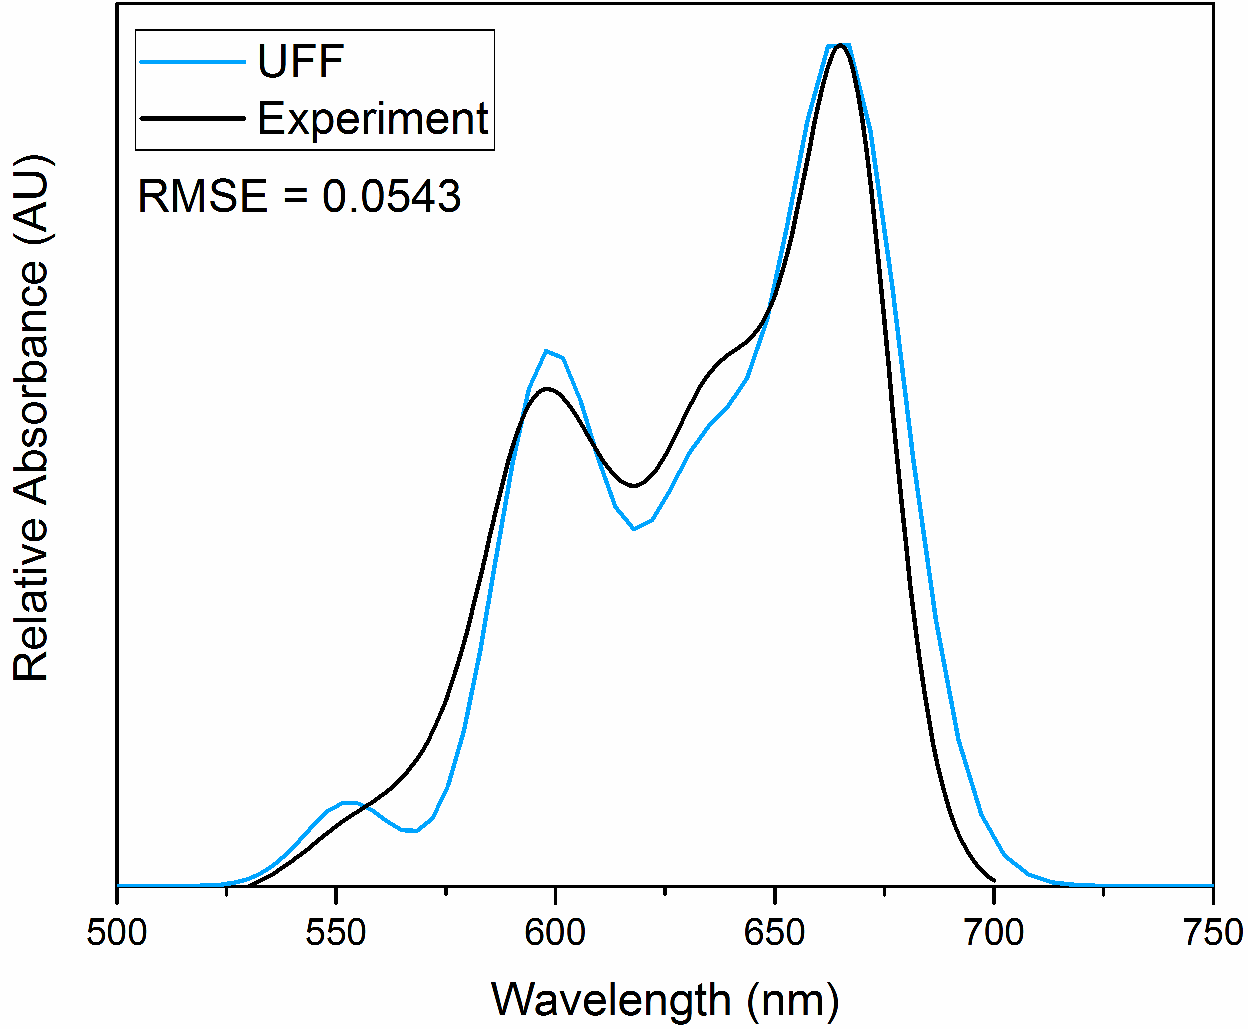
\includegraphics[width=0.8\linewidth]{figures/pub1/ob-dimerUFF.pdf}
    \caption{Theoretical absorbance spectrum generated using KRM code for the oblique dimer structure relaxed using UFF compared to experimental absorbance of oblique dimer obtained by Cannon et. al. Initial structure for oblique dimer was designed based on vectors determined by Cannon et. al., so as expected the spectra show good agreement between the theoretical and experimental \cite{Cannon2017}. RMSE value provided for quantification of difference.}\label{ob-UFF}
\end{figure}

The next stage in the investigation of the effect of DNA scaffolding is based on the simplifying assumption that the main contribution of the DNA scaffold is the position restraint imposed by the alkyl linker chains. This assumption is based on necessity (the system is too large for DFT) and the observation the absorbance of the monomer does not change appreciably when bound to DNA (see \autoref{spectra-free-bound}). After relaxation in DNA with UFF, the oblique dimer with fixed linker chains was optimized using PM6 and then DFT using the 6-31+G(d,p) basis set (chosen based on the results of the H-dimer calculations which showed that the BSSE using this basis set for the Cy5 dimers was not significant) and various hybrid functionals (B3LYP, CAM-B3LYP, and $\omega$B97XD). \autoref{ob-all} shows the predicted spectra of the relaxed structures using the KRM code. For the corresponding orientation of the dyes after relaxation, see \autoref{tab:ob-orientation}. 
\begin{figure}[h!]
    \centering
    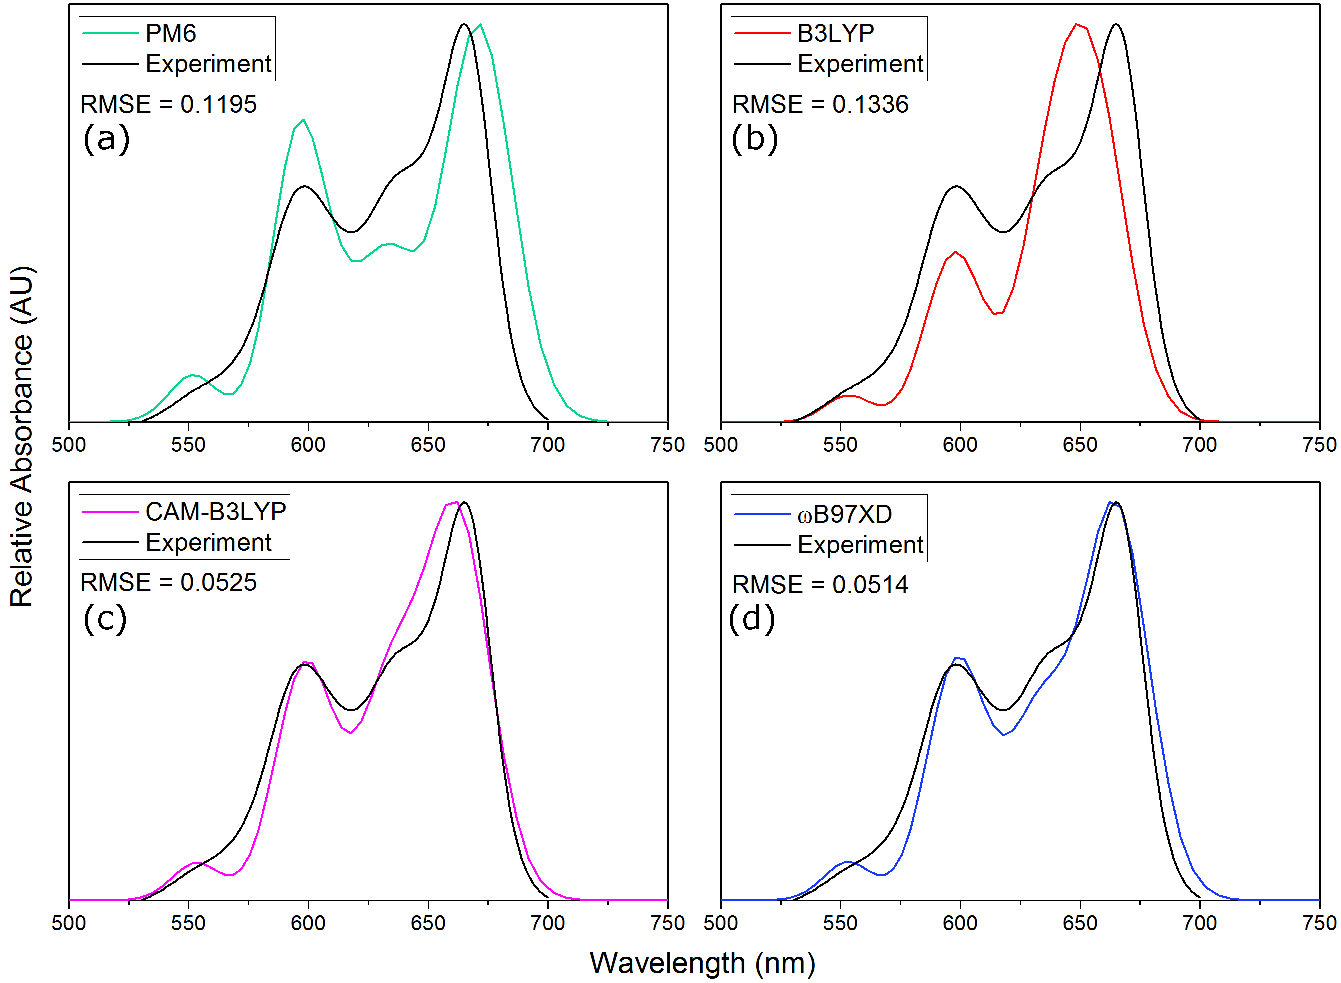
\includegraphics[width=0.8\linewidth]{figures/pub1/obdimer-all-ad.pdf}
    \caption{Theoretical absorbance spectra for the relaxed oblique dimer generated using KRM code compared to experimental absorbance of oblique dimer obtained by \cite{Cannon2017}. All structures were relaxed with the (a) PM6 semi-empirical method before further relaxation with a hybrid functional: (b) B3LYP, (c) CAM-B3LYP, or (d) $\omega$B97XD. RMSE value provided for quantification of difference.}\label{ob-all}
\end{figure}

The small peak at 550 nm in all predicted spectra corresponds to a vibronic transition which is not observed in experiment most likely due to temperature or solvent induced peak broadening. Comparison of the predicted spectra in \autoref{ob-all} with the experimental spectra suggest that the dimer drifts away from the orientation found by experiment after (a) the PM6 optimization (the RMSE value increases from 0.0543 to 0.1195) and drifts even further upon optimization using (b) B3LYP (the RMSE value increases from 0.1195 to 0.1336); however, after optimization with the long range corrected (c) CAM-B3LYP and dispersion corrected (d) $\omega$B97XD functionals, the predicted spectra become a better fit to the experimental spectrum (the RMSE decreases from 0.1195 to 0.0525 and 0.0514 for CAM-B3LYP and $\omega$B97XD, respectively), and even show a better agreement with the experimental spectrum than the initial position which was designed to be a good fit (\autoref{ob-UFF}, RMSE=0.0543). Although the KRM method requires reducing the molecules to vectors and does not involve any ab-initio energy calculations from atomic positions, this result suggests that long-range and dispersion correction are vital to accurately modelling the intermolecular interactions of the dye aggregates. Additionally, this system was also optimized using dispersion corrected B3LYP, but analysis of the resulting structures with the KRM code suggests they are not as good a fit to experiment \cite{Grimme2006, Grimme2011} (see \autoref{spectra-d2d3}). The structure of the oblique dimer optimized using $\omega$B97XD, which provides the best fit of the predicted spectrum using the KRM code to the experimental spectrum, is shown in \autoref{ob-structure}.
\begin{figure}[h!]
    \centering
    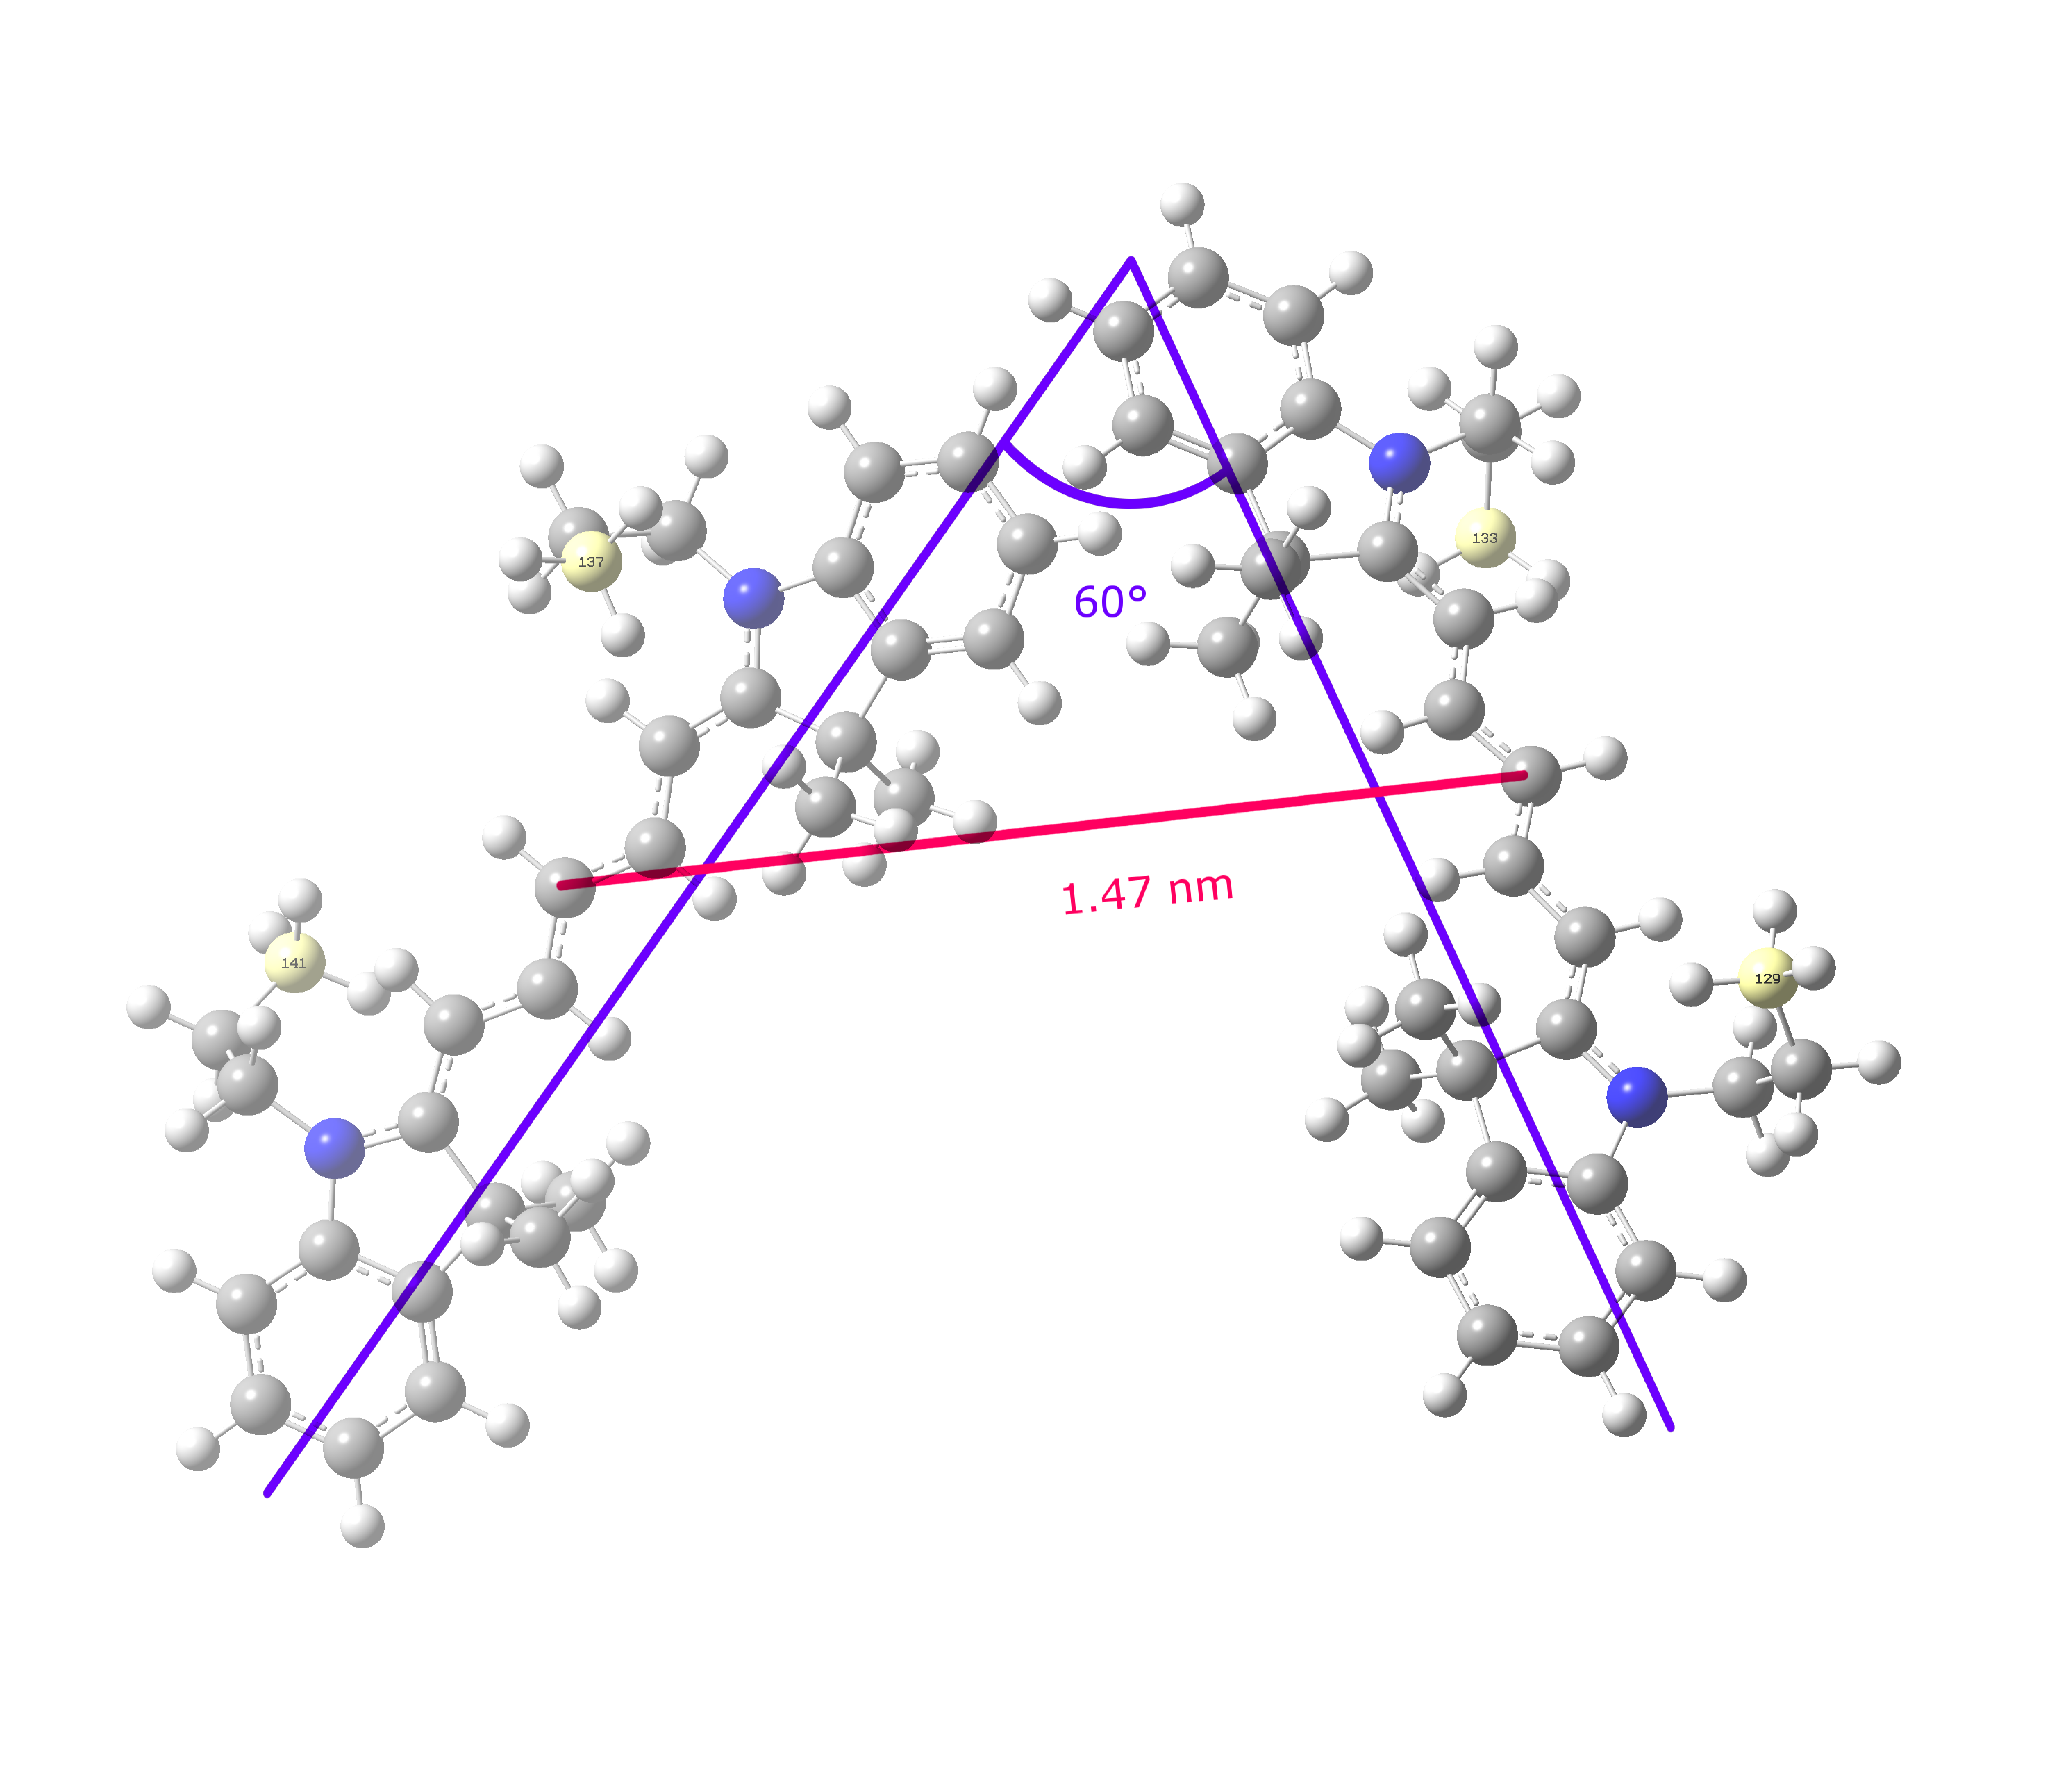
\includegraphics[width=0.8\linewidth]{figures/pub1/obdimer3-top.pdf}
    \caption{Structure of the Cy5 oblique dimer with propyl linkers optimized using $\omega$B97XD functional. The terminal carbon atoms of the linker chain (highlighted in yellow) were “frozen” during relaxation. See \autoref{ob-all}(d) for the predicted spectrum from this structure using the KRM code.}\label{ob-structure}
\end{figure}

In addition to the spectra generated using the KRM code, an ab-initio calculation of the absorbance spectrum of the monomer was performed using the Franck-Condon approximation with and without the Herzberg-Teller approximation on vibrational modes determined using DFT and TD-DFT (see \autoref{cy5-structure} for molecular structure). The intensity of absorption depends on the square of the electronic transition dipole moment and the radiation frequency, and it is also assumed that the Born-Oppenheimer approximation, where nuclear motions are much slower than electronic transitions, holds true, so during an electronic transition the nuclei can be considered static \cite{Born2000}. The Franck-Condon (FC) approximation further assumes that the electronic transition dipole also remains static, while the Herzberg-Teller (HT) approximation allows for linear variation of the dipole moment with respect to the nuclear coordinates during the transition \cite{Franck1926a, Condon1926, Santoro2007, Santoro2008}. The FC approximation can predict fully dipole-allowed transitions while the HT approximation can better predict weakly allowed or dipole forbidden transitions. \autoref{tab:max-abs} shows the shift in absorption maxima (relative to experiment) for spectra generated using the FC and FC with HT approximations. 
\begin{figure}[h!]
    \centering
    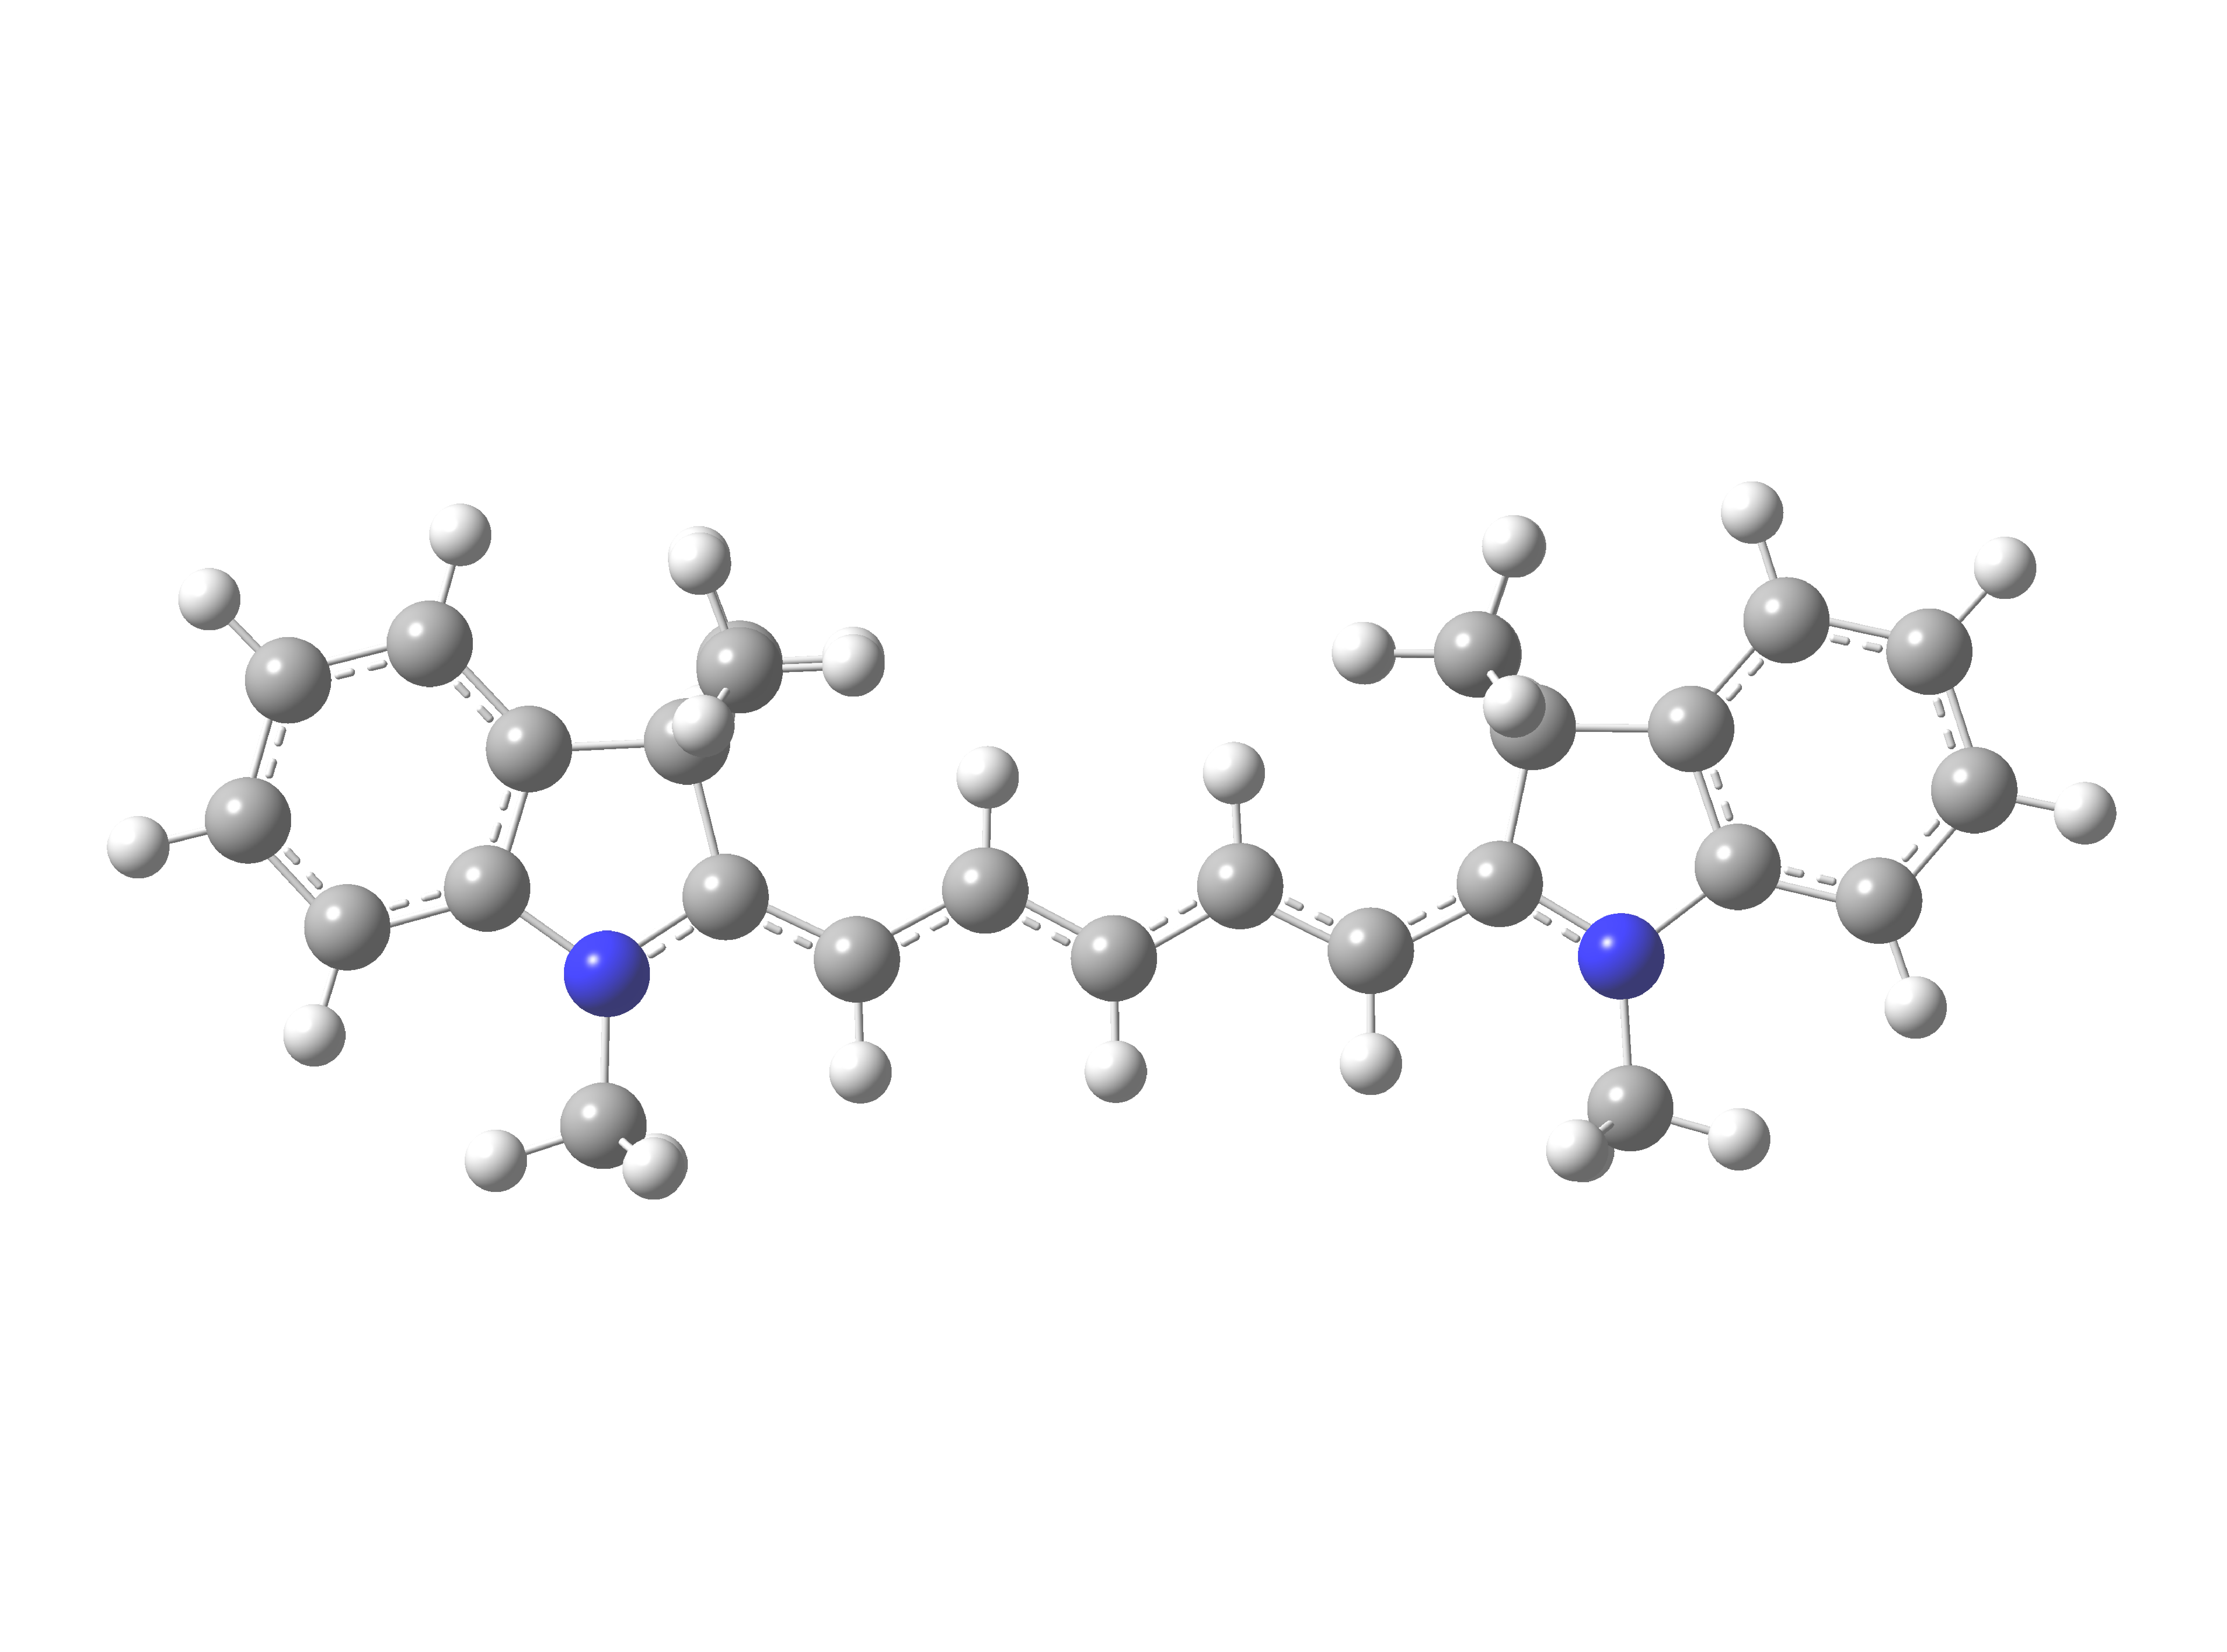
\includegraphics[width=0.8\linewidth]{figures/pub1/cy5-B3LYP.pdf}
    \caption{Molecular structure of Cy5 monomer optimized using 6-31+G(d,p) B3LYP in IEF-PCM water solvent. The average C=C bond length in the methine chain is 1.4 \AA. }\label{cy5-structure}
\end{figure}

\begin{table}[h]
\centering
\caption{Comparison of the difference in maximum absorbance ($\Delta\lambda_{max}$) of experimental Cy5 monomer spectrum \cite{Cannon2017} to absorption spectra generated using the Franck-Condon (FC) approximation with or without contribution from the Herzberg-Teller (HT) approximation. Approximation schemes use TD-DFT and DFT results relaxed using the 6-31+G(d,p) basis set and three different xc-functionals in IEF-PCM (water) solvent.} \label{tab:max-abs}
\begin{tabular}{llc}
\hline
xc-functional & Approximation & $\Delta\lambda_{max}$ (eV) \\ \hline
B3LYP & FC & 0.007 \\ 
B3LYP & FCHT & 0.080 \\ 
CAM-B3LYP & FC & 0.188 \\ 
CAM-B3LYP & FCHT & 0.207 \\ 
$\omega$B97XD & FC & 0.215 \\
$\omega$B97XD & FCHT & 0.222 \\ 
\end{tabular}
\end{table}

Although the optimized geometries of the Cy5 monomers do not vary appreciably between exchange-correlation functionals (see \autoref{tab:structure}), the transition energies from the ground to excited state are found to depend strongly on the optimization conditions. \autoref{tab:max-abs} and \autoref{spectra-fc-pcm} show that the conditions which bring the wavelength of maximum absorbance, $\lambda_{max}$, of the predicted spectrum closest to that observed in experiment are obtained using the Franck-Condon approximation on structures optimized with the B3LYP functional in IEF-PCM water solvent ($\Delta\lambda_{max}$x 0.007 eV or 2.2 nm). The consideration of long-range (CAM-B3LYP) and dispersion correction ($\omega$B97XD) overestimate the ground to excited state energy transition of the monomer. 
\begin{figure}[h!]
    \centering
    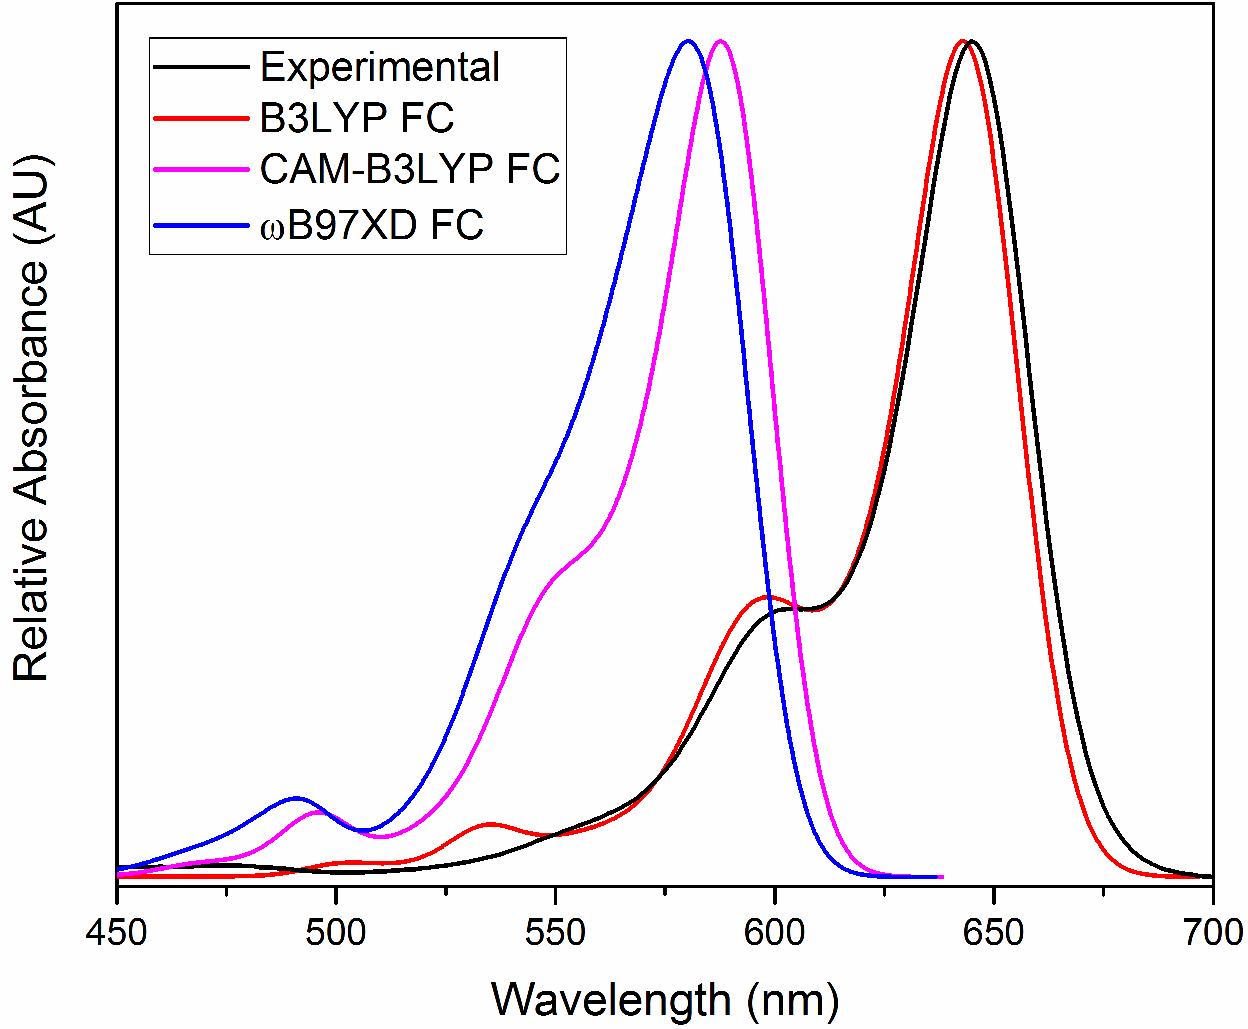
\includegraphics[width=0.8\linewidth]{figures/pub1/FC-PCM.pdf}
    \caption{Comparison of spectra generated using the FC approximation to experimental spectrum obtained by \cite{Cannon2017}. The almost complete overlap of the predicted absorbance spectrum generated using B3LYP and the FC approximation (red line) with the experimental spectrum (black line) suggest that the conditions not only accurately predict $\lambda_{max}$ but also the vibronic structure. All structures were optimized using 6-31+G(d,p) basis set in IEF-PCM (water) solvent.}\label{spectra-fc-pcm}
\end{figure}

For all spectra the predicted energies of the transitions are higher than observed in experiment. This is expected; TD-DFT using hybrid functionals has been shown to overestimate the vertical absorbance transition energy of cyanine dyes \cite{Laurent2014, Champagne2006, LeGuennic2015}. The addition of solvent is known to improve the prediction of the transition energy \cite{Champagne2006} and appears to red-shift the energies and improve the calculation of the most intense transition, $\lambda_{max}$, for all xc-functionals regardless of whether only the FC or also the HT approximations are considered. (See \autoref{spectra-vac} for spectra from vacuum calculations.) \autoref{spectra-fc-pcm} provides a comparison of the Cy5 monomer spectra generated with various exchange-correlation functionals in IEF-PCM water solvent using the FC approximation. The good agreement between the absorbance spectrum generated using the B3LYP exchange-correlation functional with the FC approximation and the experimental spectrum shows that not only does this method accurately predict $\lambda_{max}$, but the relative strength of the vibronic peaks also seem to be in good agreement. 

The use of the HT approximation does not improve the calculation of the most intense transition which suggests that the contribution of weakly-allowed or dipole-forbidden transitions to the absorption spectrum of a Cy5 molecule is negligible. \autoref{spectra-fcht-pcm} compares the spectra for the same structures generated using the FC approximation with the HT approximation and shows that this method is not as useful for predicting the absorption spectrum for this system as the FC approximation alone. As opposed to the HT principle, using the FC principle the symmetric ground state vibration can only couple with symmetric vibrations; the intensity distribution of the band shapes will be dominated by one vibrational mode \cite{Mustroph2018}. The good agreement of the absorbance spectrum generated using the FC principle with experiment suggests that primarily one vibrational mode contributes to the vibrational profile of Cy5. 
\begin{figure}[h!]
    \centering
    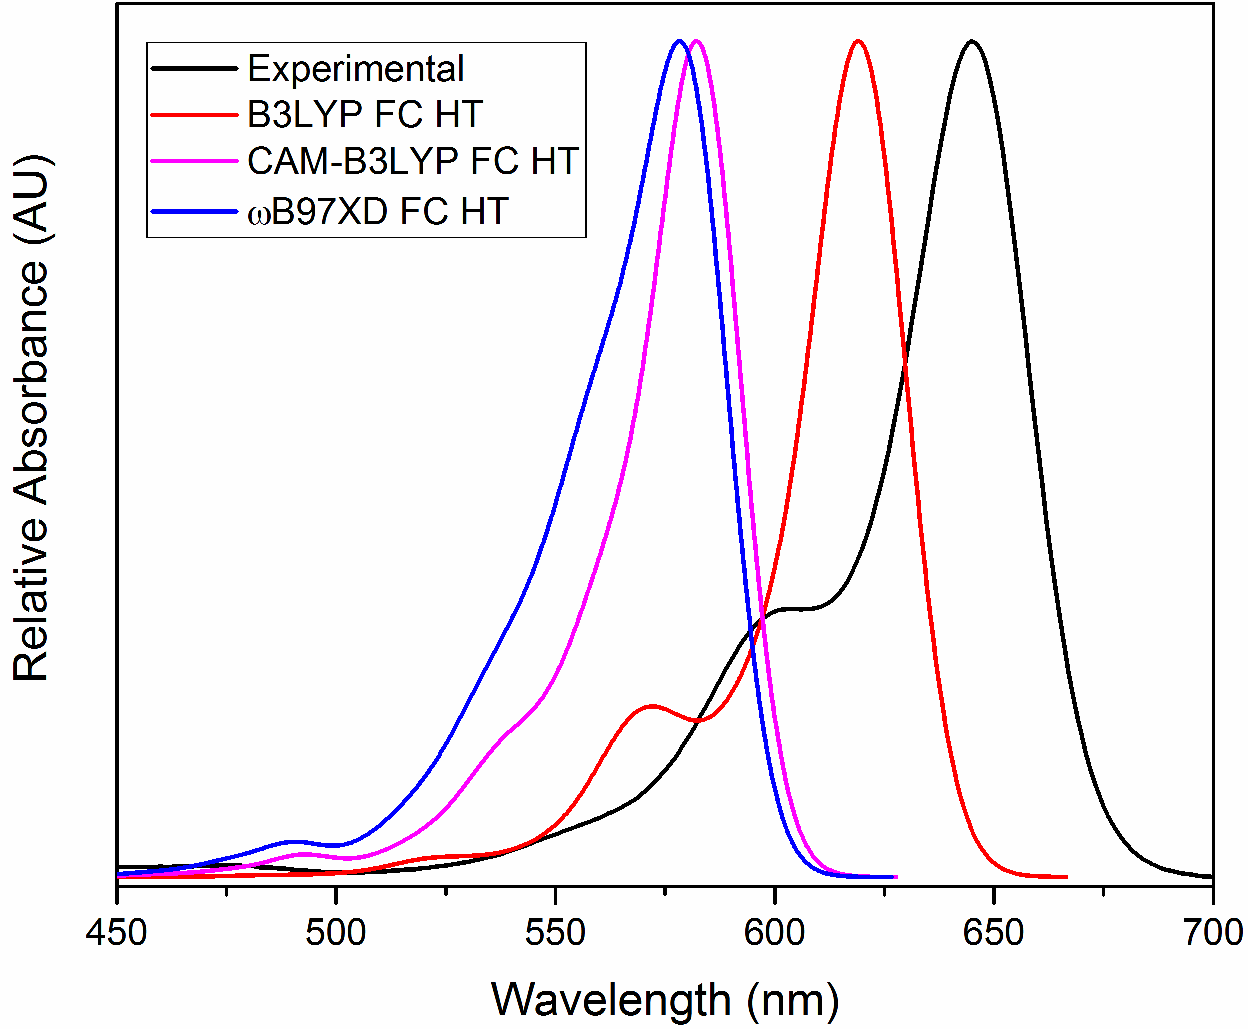
\includegraphics[width=0.8\linewidth]{figures/pub1/FCHT-PCM.pdf}
    \caption{Comparison of spectra generated using the FC approximation with the HT approximation to experimental spectrum obtained by \cite{Cannon2017}. Comparison of these spectra with those in \autoref{spectra-fc-pcm} show that adding the HT approximation does not improve accuracy. All structures were optimized using 6-31+G(d,p) basis set in IEF-PCM (water) solvent.}\label{spectra-fcht-pcm}
\end{figure}

\section{Conclusions}

Comparison of the H-dimer structures within different exchange-correlation functionals shows that the structures optimized using the smaller 6-31+G(d,p) basis set are not significantly impacted by BSSE. By comparing the spectra calculated using the in-house KRM code with the experimental dimer spectrum, the oblique dimer structure optimized using the $\omega$B97XD functional in IEF-PCM water solvent provides the best agreement with the experiment. It suggests that the long-range and dispersion corrections imposed by the exchange-correlation functional are needed to accurately estimate the dye-dye interactions. Comparison of the vibrationally resolved electronic absorption spectra of the monomer produced using the FC and HT approximations shows that the spectrum obtained using the structures optimized with the B3LYP functional in IEF-PCM water solvent and the FC approximation agrees well with the experimental monomer spectrum. The B3LYP functional works well for a single molecule while the long-range and dispersion correction could over-estimate the transition energy for a single molecule. For future work, we will combine quantum mechanical and molecular mechanical (QM/MM) calculations to incorporate DNA into the chromophore system. We will also calculate vibrationally resolved absorption spectra of the oblique dimer structures to continue revealing the effect of exchange-correlation functional. Our work aims to investigate the effects that various simulation conditions have on the unobservable atomic structures and, in turn, the effects that the atomic structure has on the observable spectra. By understanding what factors are most important when simulating the system, we hope to contribute our understanding to the knowledge of how to best optimize this system in experiment.

\section{Associated Content}
\subsection{Supporting information}
The following files are available free of charge:
Molecular structure files for oblique dimers relaxed with UFF, PM6, B3LYP, CAM-B3LYP, and $\omega$B97XD. (obdimer-UFF.pdb, obdimer-PM6.pdb, obdimer-B3LYP.pdb, obdimer-CAM-B3LYP.pdb, obdimer-wB97XD.pdb)
Information about calculations including counter ions and additional dispersion corrected xc-functionals; tabulated orientation vectors and centers of mass for the H- and oblique dimers, and spectra predicted using the KRM code for the H-dimers; information about vector fitting; comparison of the absorbance spectrum of free and bound Cy5; tabulated structural information for Cy5 monomer; comparison of Cy5 monomer spectra obtained without solvent model to experimental spectrum obtained by \cite{Cannon2017} (\autoref{chap:ab-initio-SI})

\section{Author Information}
\subsection{Corresponding Author}
*Boise State University C/O Lan Li, 1910 University Drive, Boise, ID 83725-2090
\href{mailto:lanli@boisestate.edu}{lanli@boisestate.edu}

\subsection{Author Contributions}
The manuscript was written through contributions of all authors. All authors have given approval to the final version of the manuscript. 

\section{Acknowledgements}

The research was supported by National Science Foundation INSPIRE Grant No. 1648655. We would like to acknowledge the efforts of Dr. Brittany L. Cannon, Lance Patten, Allison Christy, and Donald Kellis, who provided their absorbance data and a basis for study of this system. We would like to thank our research group members, Matt Lawson, Ember Sikorski, and Thiago da Silva, for their support and helpful discussions of DFT theory. We would also like to thank Dr. Matt King and Sean Ruettgers for helpful discussion of Gaussian software and DFT theory. This research made use of the resources of the High Performance Computing Center at Idaho National Laboratory, which is supported by the Office of Nuclear Energy of the U.S. Department of Energy and the Nuclear Science User Facilities under Contract No. DE-AC07-05ID14517.  We would like to acknowledge high-performance computing support of the R2 computer cluster (DOI: 10.18122/B2S41H) provided by Boise State University’s Research Computing Department.

\section{Abbreviations}
DFT density functional theory; TD-DFT time-dependent density functional theory; KRM Kühn, Renger, and May; BSSE basis set superposition error; IEF-PCM integral equation formalism polarizable continuum model; UFF universal force field; FC Franck-Condon; HT Herzberg-Teller; HWHM half-width at half-maximum; RMSE root mean square error; QM/MM quantum mechanical and molecular mechanical; CD circular dichroism
